\NeedsTeXFormat{LaTeX2e}

\documentclass[12pt]{article}

\usepackage{amsmath}

% The above lines establish the type of LaTeX you're using, the font and the general
% type of document (article, book, letter).


% Various bold symbols - optional stuff
\providecommand\bnabla{\boldsymbol{\nabla}}
\providecommand\bcdot{\boldsymbol{\cdot}}
\newcommand\etb{\boldsymbol{\eta}}

% For multiletter symbols - optional stuff
\newcommand\Imag{\mbox{Im}} % cf plain TeX's \Im
\newcommand\Ai{\mbox{Ai}}            % Airy function
\newcommand\Bi{\mbox{Bi}}            % Airy function


% array strut to make delimiters come out right size both ends
\newsavebox{\astrutbox}
\sbox{\astrutbox}{\rule[-5pt]{0pt}{20pt}}
\newcommand{\astrut}{\usebox{\astrutbox}}

% optional shortcuts defined with \newcommand command
\newcommand\p{\ensuremath{\partial}}
\newcommand\tti{\ensuremath{\rightarrow\infty}}
\newcommand\kgd{\ensuremath{k\gamma d}}
\newcommand\shalf{\ensuremath{{\scriptstyle\frac{1}{2}}}}
\newcommand\sh{\ensuremath{^{\shalf}}}
\newcommand\smh{\ensuremath{^{-\shalf}}}
\newcommand\squart{\ensuremath{{\textstyle\frac{1}{4}}}}
\newcommand\thalf{\ensuremath{{\textstyle\frac{1}{2}}}}
\newcommand\ttz{\ensuremath{\rightarrow 0}}
\newcommand\ndq{\ensuremath{\frac{\mbox{$\partial$}}{\mbox{$\partial$} n_q}}}
\newcommand\sumjm{\ensuremath{\sum_{j=1}^{M}}}
\newcommand\pvi{\ensuremath{\int_0^{\infty}%
  \mskip \ifCUPmtlplainloaded -30mu\else -33mu\fi -\quad}}

\newcommand\etal{\mbox{\textit{et al.}}}
\newcommand\etc{etc.\ }
\newcommand\eg{e.g.\ }


%%%%%%%%%%%%%%%%%%%%%%%%%%%%%%%%%%%%%%%%%%%%%%%%%%%%%%%%%%%%%%

% FOR PDFLATEX:  YOU MAY NEED TO (UN)COMMENT THE FIRST LINE DEPENDING ON YOUR (PDF)LATEX DISTRO
%\newif\ifpdf\ifx\pdfoutput\undefined\pdffalse\else\pdfoutput=1\pdftrue\fi
\newcommand{\pdfgraphics}{\ifpdf\DeclareGraphicsExtensions{.pdf,.jpg}\else\fi}

\usepackage{graphicx} % Include figure files
%\usepackage{epsfig}  % old
\usepackage{bm}% bold math

\usepackage{amsfonts}
\newcommand{\field}[1]{\mathbb{#1}}
\newcommand{\C}{\field{C}}
\newcommand{\R}{\field{R}}

\def\eg{{e.g.\ }}
\def\etc{{etc.\ }}
\def\etal{\mbox{\it et al.\ }}

%%%%%%%%%%%%%%%%%%%%%%%%%%%%%%%%%%%%%%%%%%%%%%%%%%%%%%%%%%%%%%%
%%%%%%%%%%%%%%%%%%%%%%%%%%%%%%%%%%%%%%%%%%%%%%%%%%%%%%%%%%%%%%%

% \linespread{2}  UNCOMMENT this for Double Spacing; I think it looks awful.  Most values work, i.e.. 1.67

% it all starts here

\begin{document}

% \pdfgraphics

\section*{Sai Chikine \& Alex Rybchuk}  % No Section number because I used \section* not \section
                                                                           % same thing works for \equation*
\begin{align*}
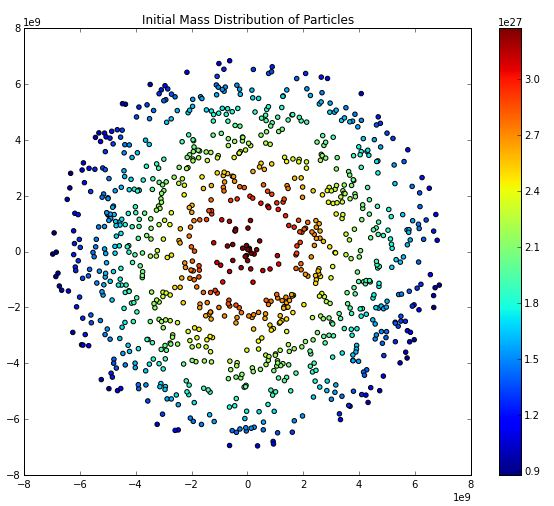
\includegraphics[width=2in]{graphic.jpg}
\end{align*}                                                                          



\section*{Jupiter Progress Report}  
Our project as of now can be separated into two parts: setting up initial conditions and iterating through force and displacement calculations.

\subsection*{Initial Conditions}
In order to collide two planets, we first have to initialize several factors. First, we initialized poisition using a radial distribution equation provided by our textbook. Next, we modeled initial densities and the pressure distribution. We were then able to fix the mass of each particle using a compact support smoothing kernel. 

\subsection*{Force \& Displacement Calculations}
These calculations have been causing us some trouble, but we have been making progress. The tried modeling the pressure gradient using a Guassian kernel, but that lead to errors, so we decided to use a compact support kernel. It looks like the pressure gradient is now being calculated correctly. Gravity is causing us issues at the moment, as not all of our particles appear to be affected by gravity, but we are currently debugging that. 

\end{document}